\section{Light and Colors}

To understand colors in computer graphics, we first have to learn about the real physical properties of colors.


\subsection{What is light?}

Light is a form of electromagnetic radiation, we perceive a very limited section of the spectrum as visible light.
\begin{center}
	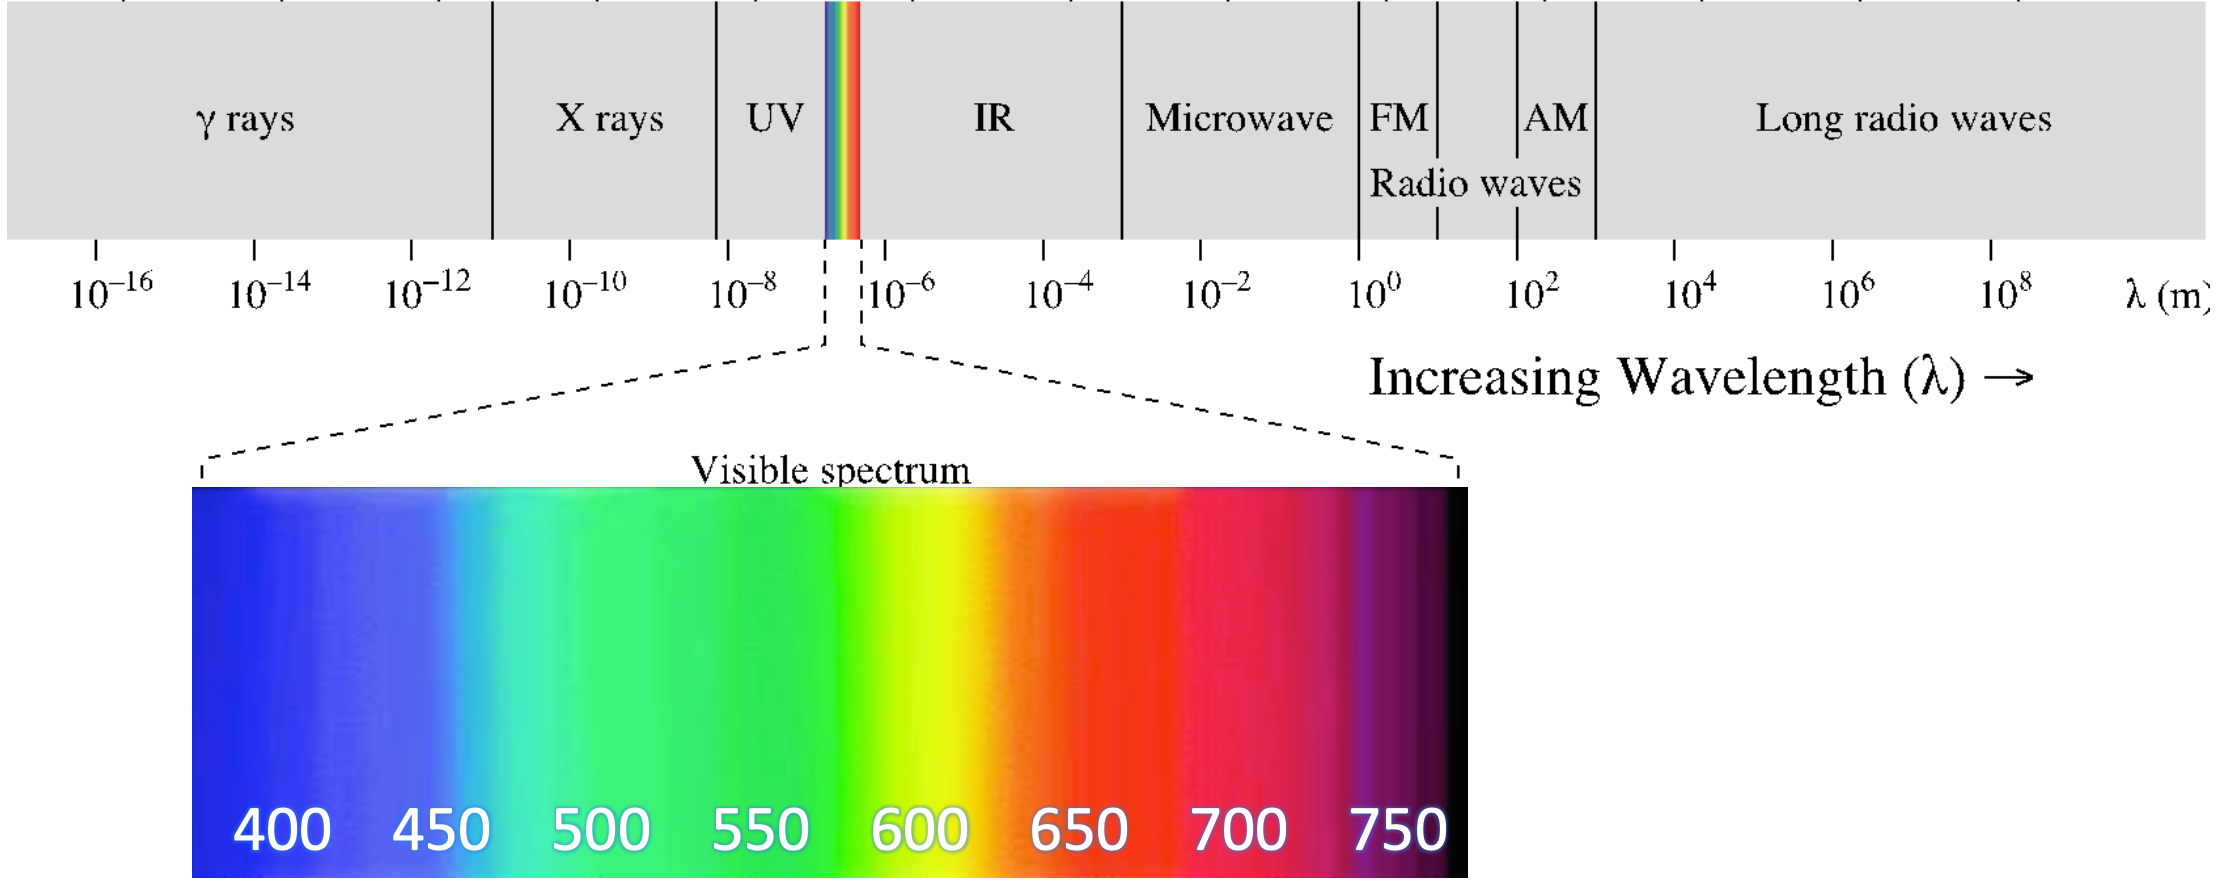
\includegraphics[width=\linewidth]{light_spectrum.png}
\end{center}

Light can be a mixture of many wavelength and is typically defined by the spectral power distribution (SPD). $P(\lambda)$ defines the intensity of this spectrum at wavelength $\lambda$. We humans then perceive this distribution as colors. A light ray carries more information than a human can process, so we project this spectrum onto a 3D subspace given by the types of cones.


\subsection{Anatomy of the Eye}  

On our retina there are two types of different cells, rods and cones. While rods respond to intensity only, the cones respond to color. There are three type of cones, each responding to a different wavelength (short = blue, medium = green, long = red). These cones are the reason we project the infinite dimensional space $P(\lambda)$ onto a 3D subspace.


\subsection{Defining the Subspace}

When doing this projection we will inherently lose some information, therefore two different SPD might look the same to us. There have been multiple attempts to standardise this subspace and the projection used. \medskip

\textbf{The CIE Primary System} \smallskip

This was one of the the first attempts at standardising the color subspace. Their approach was to try to define every color by an additive mixture of the three base colors red, green, blue. They came up with the following results:
\begin{center}
	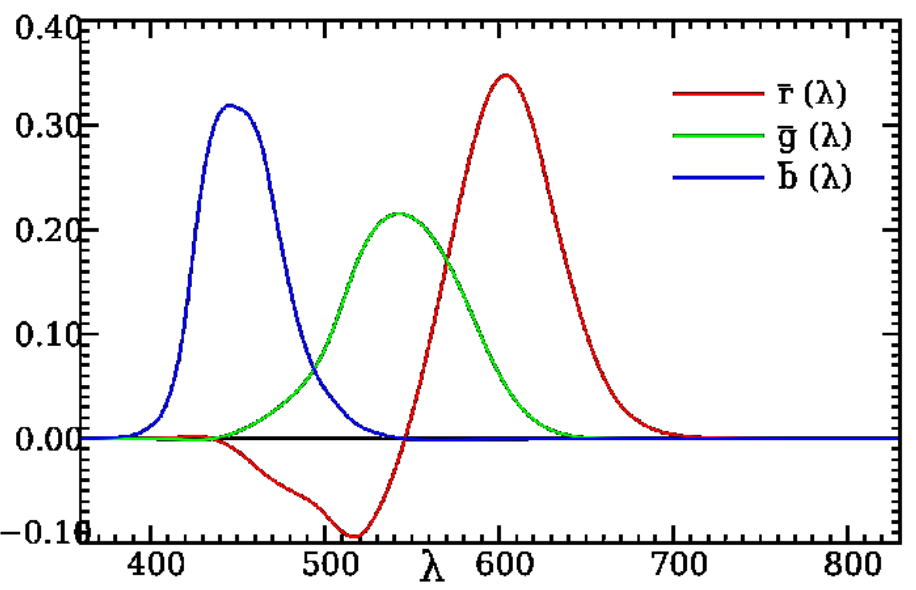
\includegraphics[width=0.8\linewidth]{rgb_mixture.png}
\end{center}

This shows that there are some colors that cannot be reproduced (negative r value). The CIE XYZ color space defines transformation from these three curves to a vector $(X, Y, Z)$. 
$$X = \int_0^\infty P(\lambda) \bar x (\lambda) d\lambda$$
$$Y = \int_0^\infty P(\lambda) \bar y (\lambda) d\lambda$$
$$Z = \int_0^\infty P(\lambda) \bar z (\lambda) d\lambda$$

The transformation matrix from RGB to XYZ is then given by:
$$\begin{pmatrix}
	\bar x(\lambda) \\
	\bar y(\lambda) \\
	\bar z(\lambda) \\
\end{pmatrix}
=
\begin{pmatrix}
	2.36 & -0.515 & 0.005 \\
	-0.89 & 1.426 & 0.014 \\
	-0.46 & 0.088 & 1.009 \\
\end{pmatrix}
\begin{pmatrix}
	\bar r(\lambda) \\
	\bar g(\lambda) \\
	\bar b(\lambda) \\
\end{pmatrix}
$$

These transformed curves have the properties that they are normalized, positive definite and the $\bar y (\lambda)$ curve corresponds to the luminance.

\begin{center}
	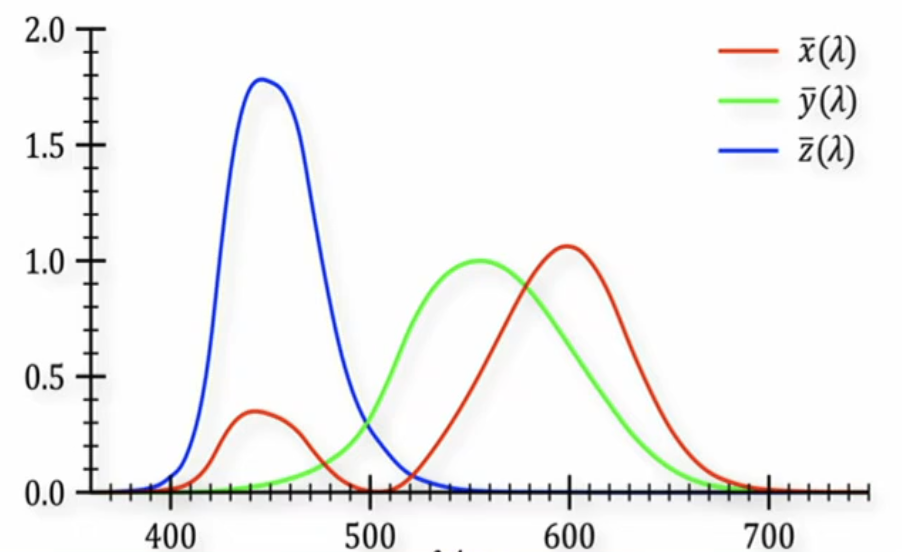
\includegraphics[width=0.8\linewidth]{XYZ.png}
\end{center}

As the XYZ color space is 3D, it is often not very practical. Therefore we normalize the XYZ components and project it into a 2D space:
$$x = \frac{X}{X + Y + Z} \qquad y = \frac{Y}{X + Y + Z}$$

Now $(x,y)$ characterize color and $Y$ characterizes brightness. If we plot $(x,y)$ on a plane, we get all the colors of a single brightness (chromaticity chart).
\begin{center}
	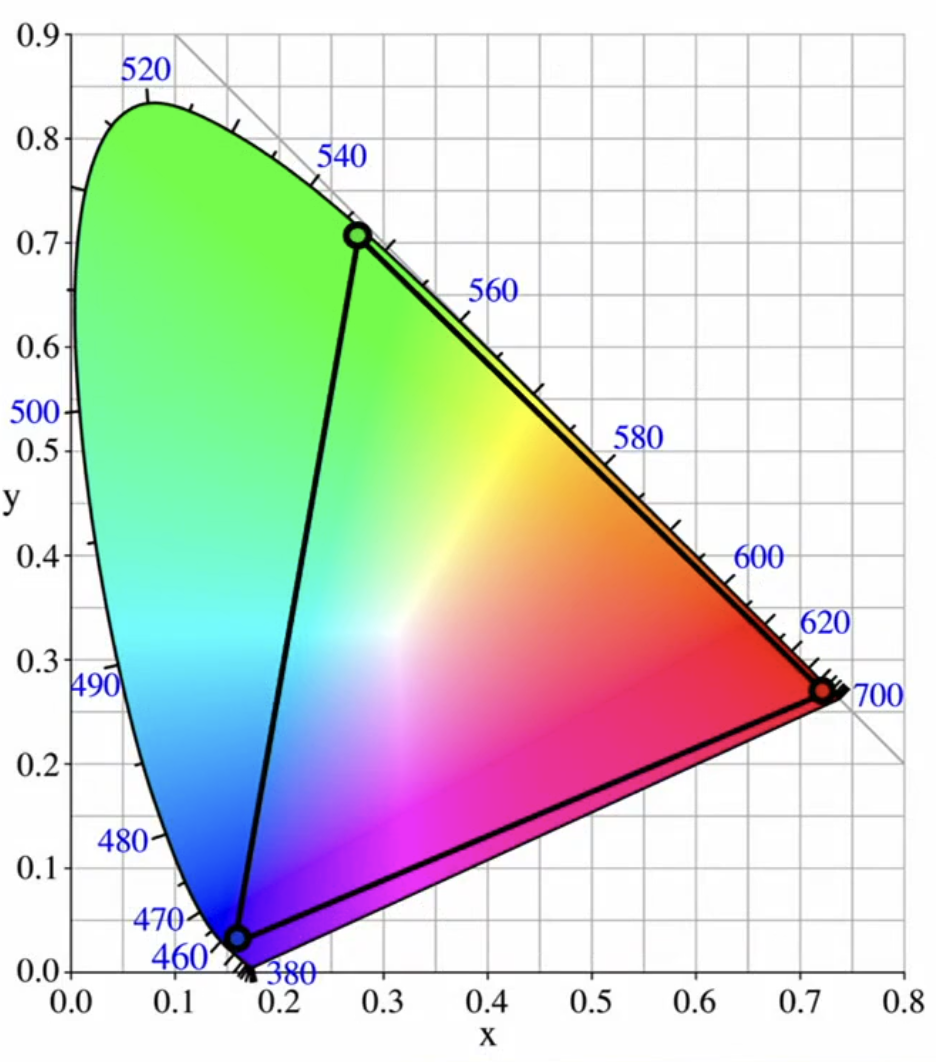
\includegraphics[width=0.65\linewidth]{horseshoe.png}
\end{center}
 
The primary colors are on the boundary of the horse shoe and all linear combinations of two colors are on a line. Screens are limited to a combination of three colors (triangle  in the chart), so they can not show all possible colors.\medskip

\textbf{Other Color Spaces}\smallskip

The \textbf{CMY color space} is the inverse of the RGB space.
$$\begin{pmatrix}
	C \\ M \\ Y
\end{pmatrix} = \begin{pmatrix}
	1 \\ 1 \\ 1
\end{pmatrix} - \begin{pmatrix}
	R \\ G \\ B
\end{pmatrix}$$

The \textbf{HSV color space} consists of hue (base color), saturation (purity of color) and value (brighness). This is a more user oriented color space, as it is rather intuitive to interact with. \medskip

\textbf{MacAdams} ellipses describe an area around a color, such that everything inside the ellipse is perceptual indistinguishable.
\begin{center}
	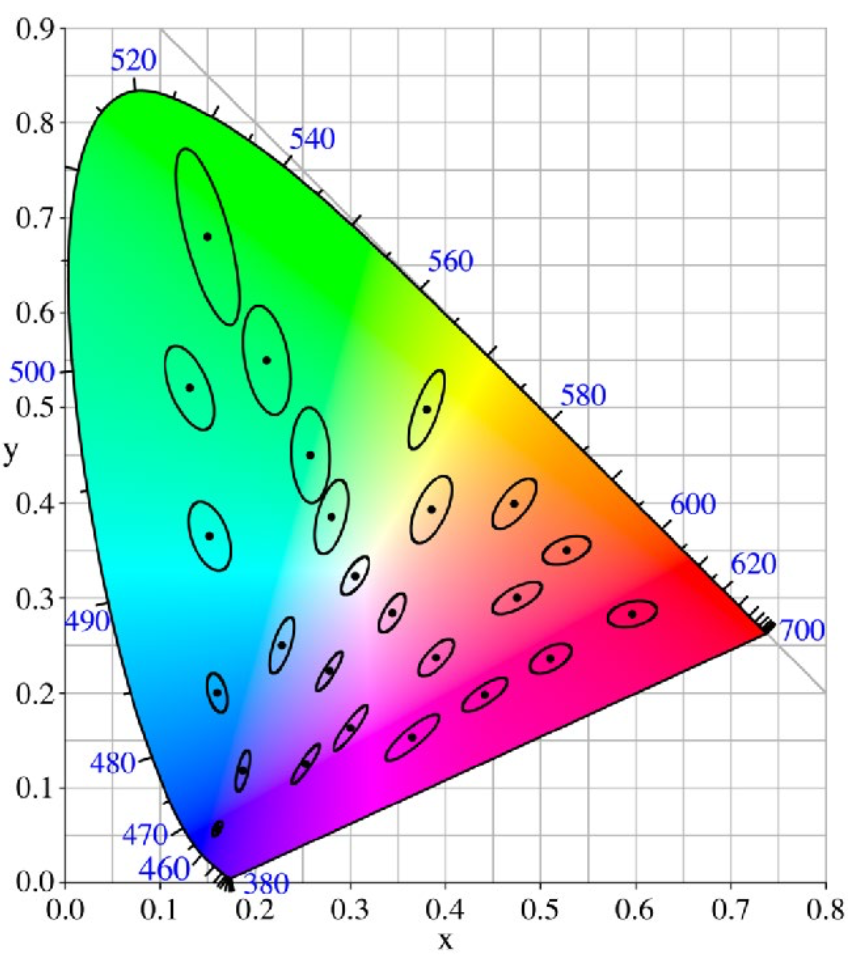
\includegraphics[width=0.5\linewidth]{macadams.png}
\end{center}

The \textbf{CIELAB and CIELUV color spaces} use MacAdams ellipses and transform the color space, so that the ellipses become nearly circular.
\begin{center}
	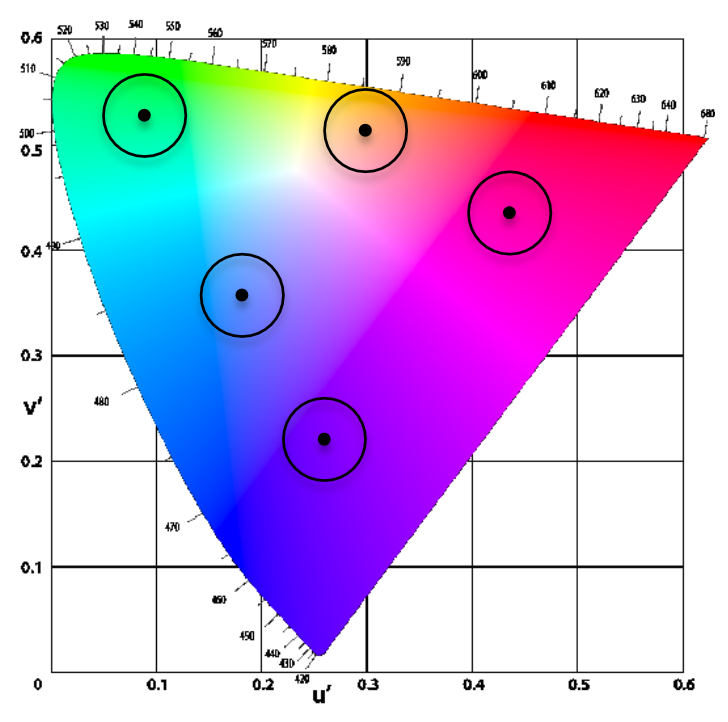
\includegraphics[width=0.5\linewidth]{cieluv.png}
\end{center}

